\section{Cours 10}\label{cours-10}

\subsection{La mémoire}\label{la-muxe9moire}

Accéder à la mémoire directement n'est pas une bonne solution car on
doit connaitre son organisation à la compilation. Impossible car si on
passe de 2 Go de RAM à 4 il faut tout recompiler !! On va virtualiser
tout ça

\subsubsection{La Mémoire Virtuelle}\label{la-muxe9moire-virtuelle}

On va devoir faire une traduction du virtuelle à physique via le
\textbf{MMU} ou \textbf{Memory Management Unit} (qui est dans le
processeur).

\begin{figure}
\centering
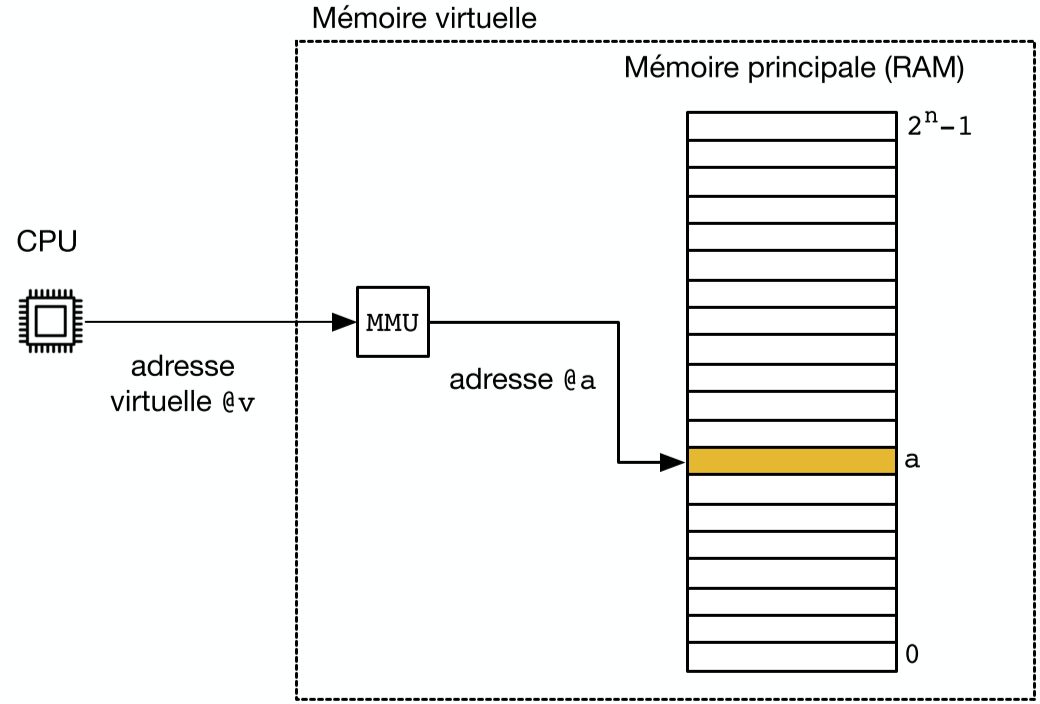
\includegraphics{image-52.png}
\caption{MMU Simple}
\end{figure}

Ainsi on peut découpler la taille et écrire les adresses sur + de 32
bits.

On peut faire de la librairie partagée très facilement, on peut voir que
2 programmes pointes vers la même zone de la RAM !

\paragraph{Avantages}\label{avantages}

On peut utiliser le stockage sur le disque pour mettre des objets
inutilisées de la RAM. C'est le principe de \textbf{\texttt{swap}}. Et
on peut faire vice-versa.

\subsubsection{Fonctionnement de la mémoire
Virtuelle}\label{fonctionnement-de-la-muxe9moire-virtuelle}

La mémoire a un accès par \emph{adresse} et les SSD par \emph{secteur}.
La mémoire virtuelle est divisée par \textbf{pages}. C'est une zone de
mémoire \textbf{contiguë} de taille 4 Ko (4096 octets (on peut vérifier
via \texttt{getpagesize()})).

On a toujours un nombre entier de pages. De plus, chaque segment (les 6)
occupe leurs propres pages.

Ainsi, les pages virtuelles peuvent être placées dans n'importe quelle
zone (\emph{frame}/cadre de page) de la mémoire physique.

Adresse Virtuelle est composée de:

\begin{itemize}
\tightlist
\item
  Numéro de la page
\item
  Offset sur cette page à faire
\end{itemize}

Le MMU se charge de la traduction.

\begin{figure}
\centering
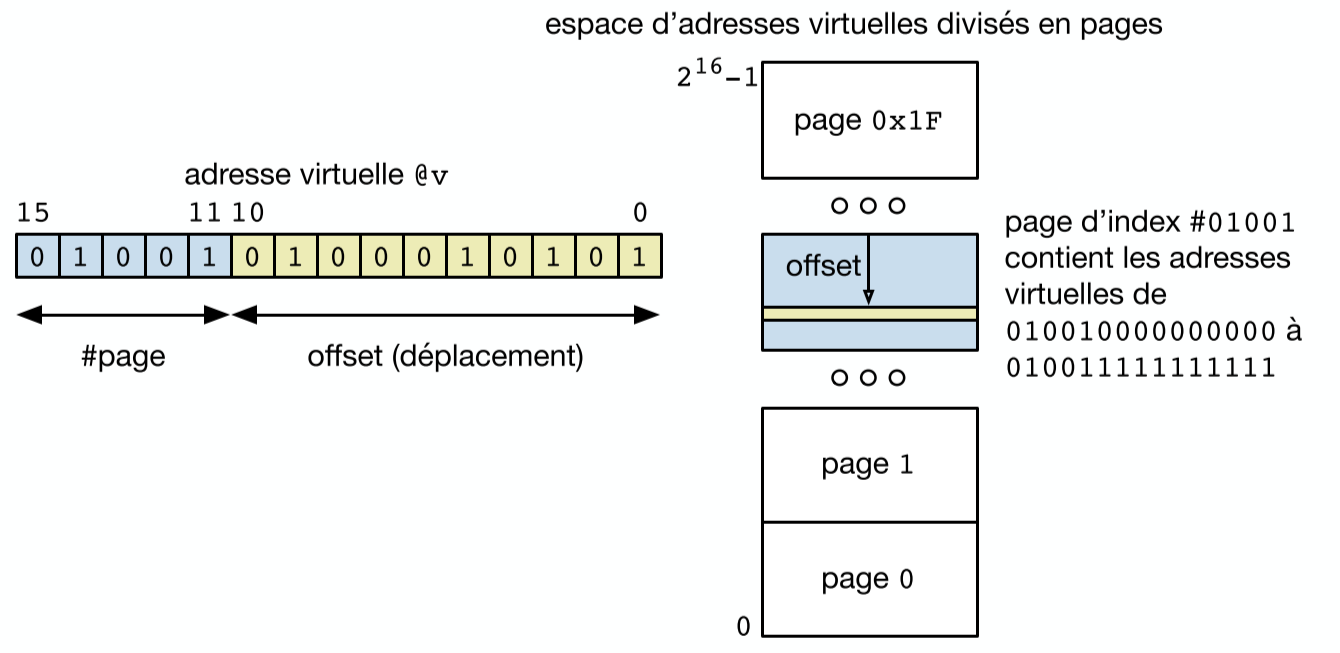
\includegraphics{image-53.png}
\caption{Découpage en page}
\end{figure}

\subsubsection{Mise en Oeuvre de la
Traduction}\label{mise-en-oeuvre-de-la-traduction}

Il doit avoir accès à l'allocation actuelle entre pages virtuelles et
cadres de pages physique. On va utiliser une table des pages:

\begin{itemize}
\tightlist
\item
  Tableau indexé par le numéro de page
\item
  Bit de validité si la page existe dans l'espace mémoire du
  \emph{processus}
\item
  Si valide: ligne du tableau indique le lien vers le numéro de cadre de
  page.
\end{itemize}

\begin{figure}
\centering
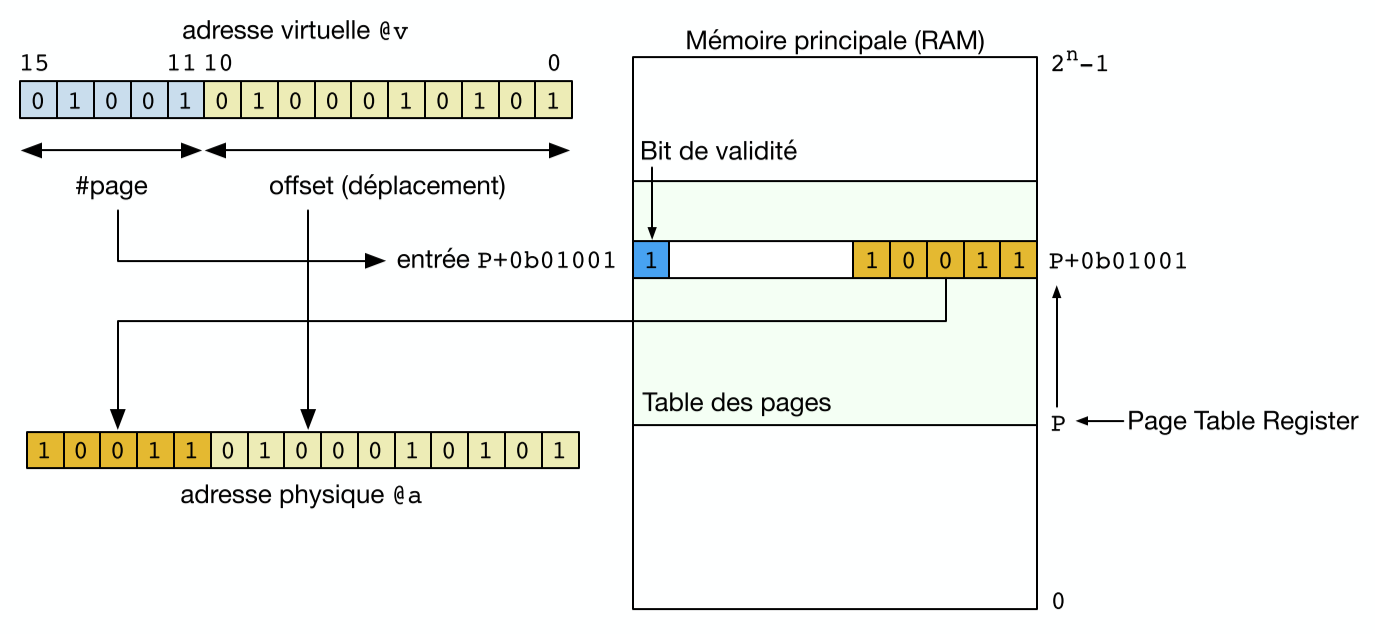
\includegraphics{image-54.png}
\caption{Traduction}
\end{figure}

Chaque processus possède donc sa \textbf{propre table des pages} (pas
pour le kernel). On a un registre spécial qui contient l'adresse de base
en mémoire de la table des pages du processus actuel (restauré à chaque
rétablissement de contexte).

\paragraph{Exemple pour 2 processus}\label{exemple-pour-2-processus}

Si on a un système 8 bits (RAM maximum de 256) ce qui nous donne 16
cadres de pages de 16 octets chacun. On décide d'avoir des adresses
virtuelles sur 6 bits donc un maximum de 64 octets par processus (chaque
processus va donc utiliser 4 pages --\textgreater{} 2 bits pour la page
4 pour l'offset).

Imaginons 2 processus \texttt{P1} et \texttt{P2} qui requiert 3 pages (2
pour leur text et 1 pour leur stack).

\begin{figure}
\centering
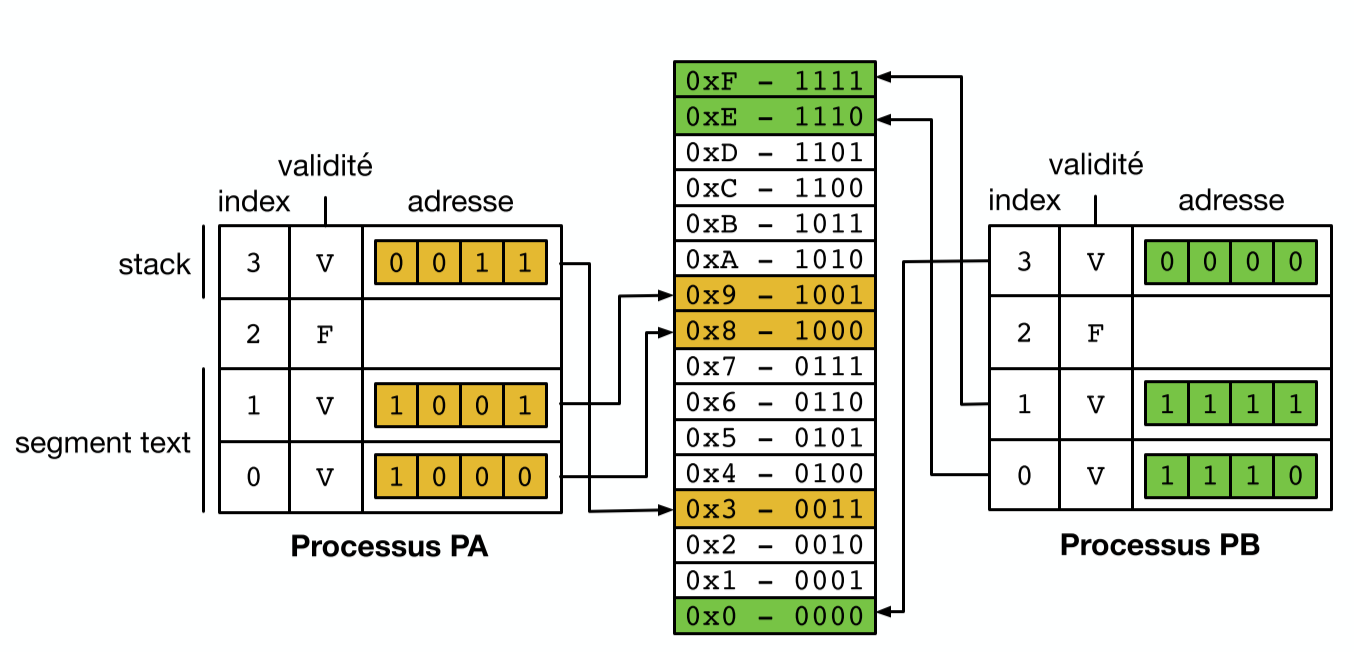
\includegraphics{image-55.png}
\caption{Exemple P1 et P2}
\end{figure}

On remarque que faire la traduction entre adresse physique et virtuelle
requiert 1 accès en plus. On va donc mettre en \emph{cache} les
traductions souvent utilisées via un \textbf{TLB} ou \textbf{Translation
Lookaside Buffer} ce qui nous donne un fonctionnement de la sorte.

\begin{figure}
\centering
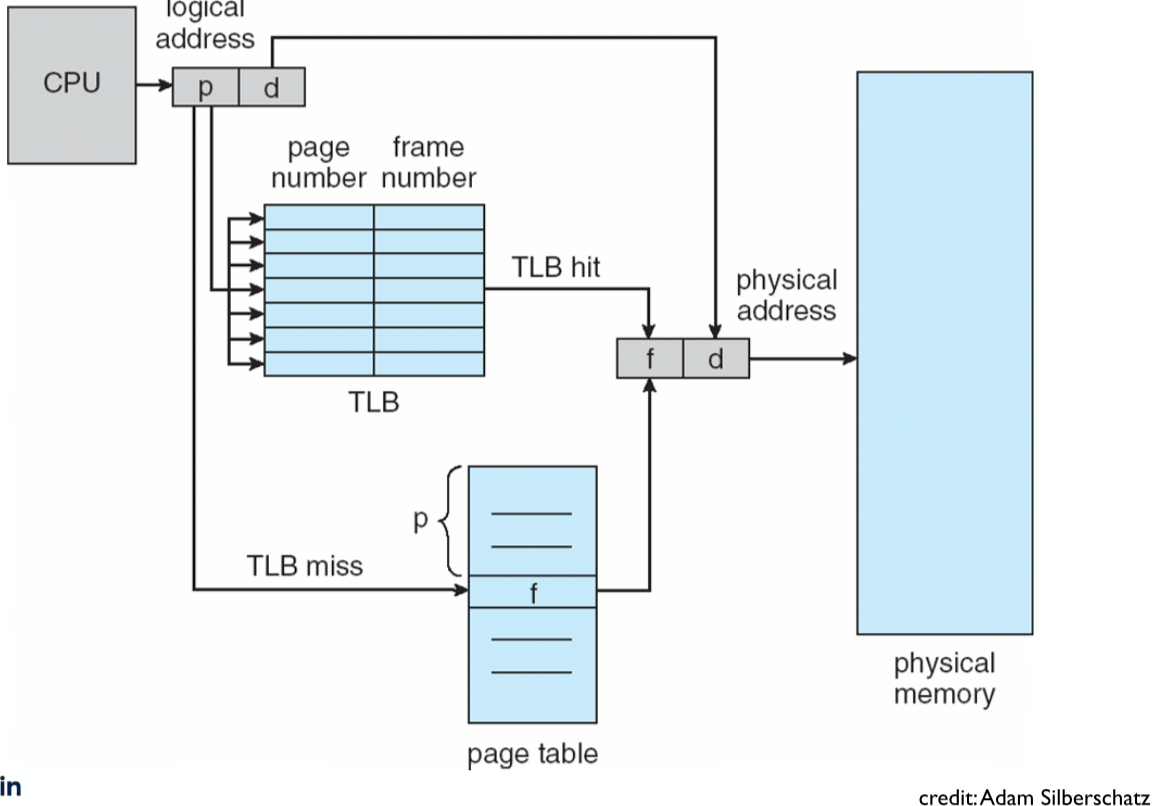
\includegraphics{image-56.png}
\caption{TLB hit et miss}
\end{figure}

\subsubsection{Protection des Pages}\label{protection-des-pages}

On peut encoder les droits d'une page sur 3 bits: \texttt{R}, \texttt{W}
et \texttt{X}. Si on essaye de faire une action invalide, on génère
ainsi un trap qui passe la main au SE.

On peut retirer des droits à une page via:

\begin{Shaded}
\begin{Highlighting}[]
\PreprocessorTok{\#include }\ImportTok{\textless{}sys/mman.h\textgreater{}}\PreprocessorTok{ }

\DataTypeTok{int}\NormalTok{ mprotect}\OperatorTok{(}\DataTypeTok{const} \DataTypeTok{void} \OperatorTok{*}\NormalTok{addr}\OperatorTok{,} \DataTypeTok{size\_t}\NormalTok{ len}\OperatorTok{,} \DataTypeTok{int}\NormalTok{ prot}\OperatorTok{);}
\end{Highlighting}
\end{Shaded}

\subsubsection{Problème du Swap}\label{probluxe8me-du-swap}

On a 2 façon de faire du swap (qui permet d'avoir plus de pages
virtuelles):

\begin{enumerate}
\def\labelenumi{\arabic{enumi}.}
\tightlist
\item
  Partition de Swap:

  \begin{itemize}
  \tightlist
  \item
    ✅ Rapide
  \item
    ❌ Portion du disque dédiée
  \end{itemize}
\item
  Fichier de Swap:

  \begin{itemize}
  \tightlist
  \item
    ✅ Flexible
  \item
    ❌ Performance moindre (fragmentation du fichier)
  \end{itemize}
\end{enumerate}

\paragraph{Fonctionnement par défaut d'un accès à une
page}\label{fonctionnement-par-duxe9faut-dun-accuxe8s-uxe0-une-page}

\begin{figure}
\centering
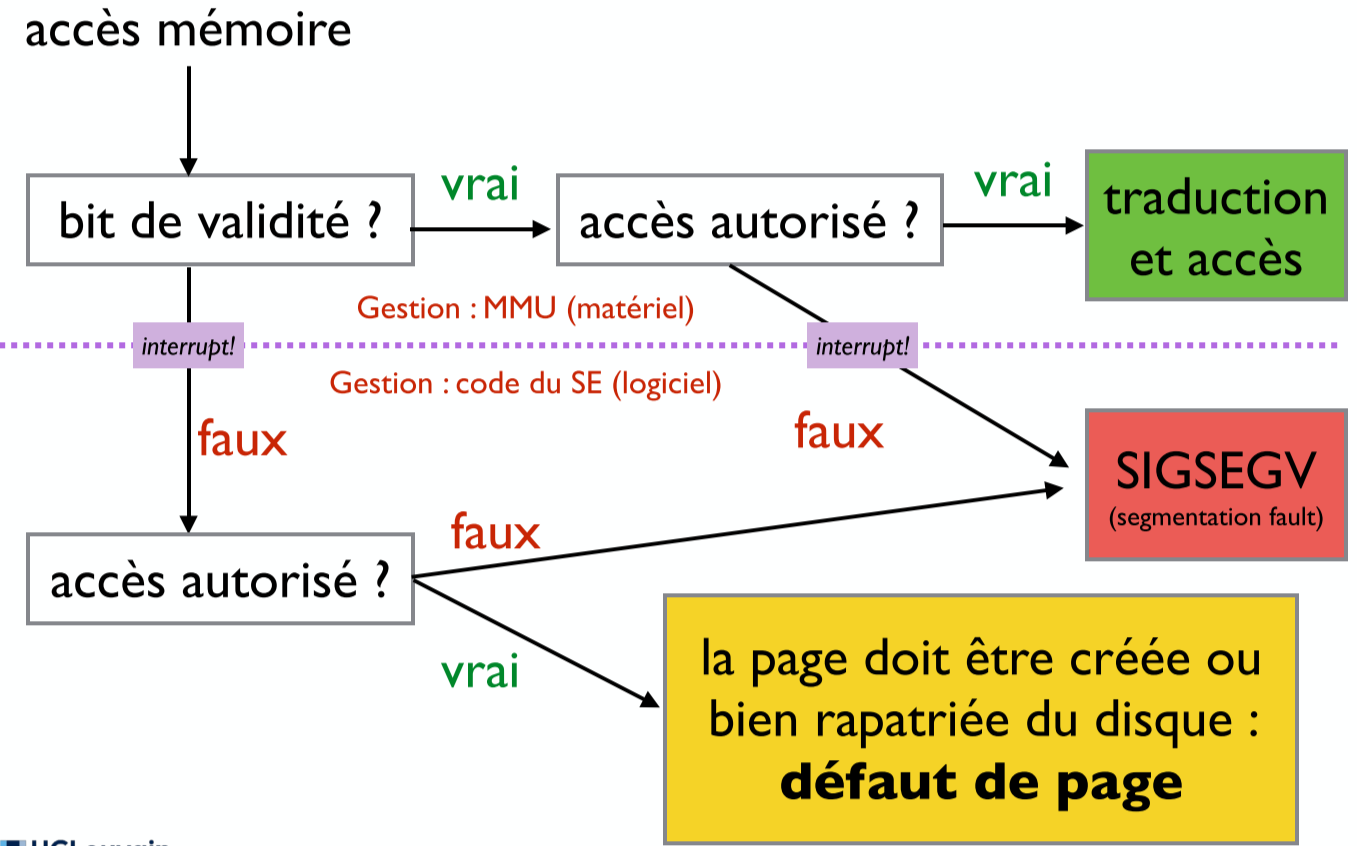
\includegraphics{image-57.png}
\caption{Défauts de page}
\end{figure}

\begin{figure}
\centering
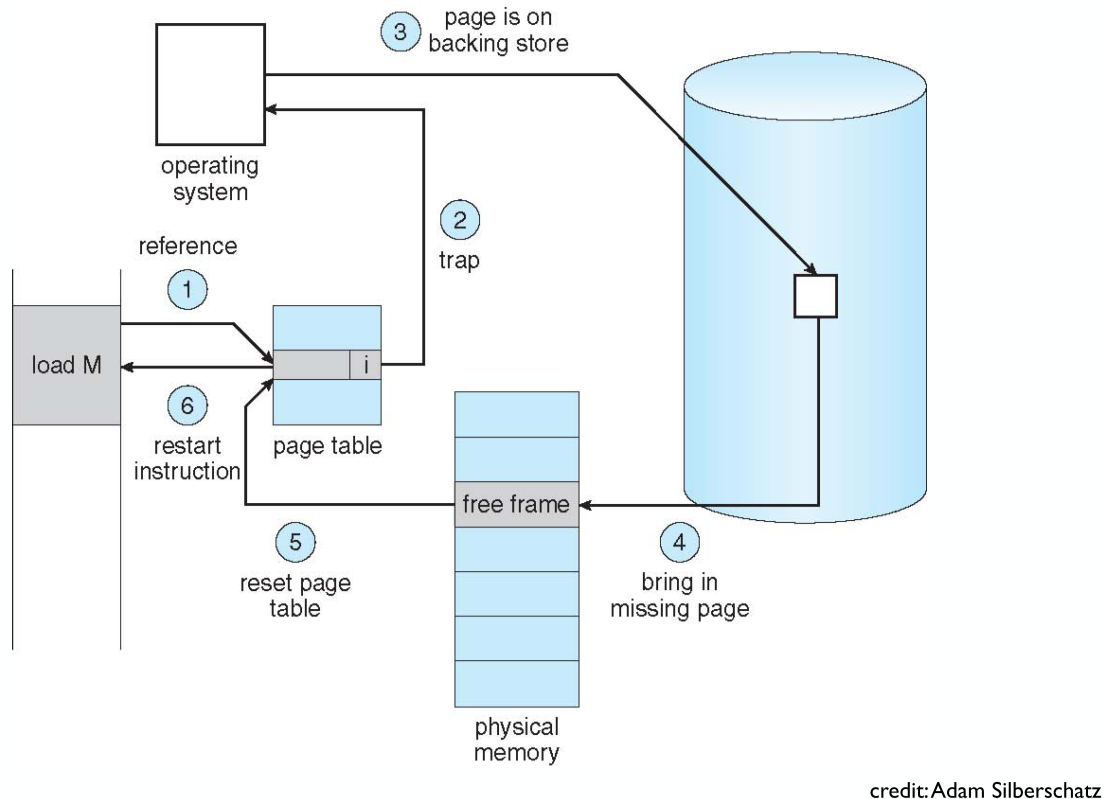
\includegraphics{image-58.png}
\caption{Traitement d'un défaut de page}
\end{figure}
